\documentclass[conference]{IEEEtran}
\IEEEoverridecommandlockouts
\usepackage{cite}
\usepackage{amsmath,amssymb,amsfonts}
\usepackage{algorithmic}
\usepackage{graphicx}
\usepackage{textcomp}
\usepackage{xcolor}
\def\BibTeX{{\rm B\kern-.05em{\sc i\kern-.025em b}\kern-.08em
    T\kern-.1667em\lower.7ex\hbox{E}\kern-.125emX}}

\usepackage{float}
\begin{document}

\title{Layer-Wise Attribute Sensitivity in Deep Models for Color and Texture Pattern Classification\\
\thanks{}
}

%\author{\IEEEauthorblockN{Anonymous Authors}}

\author{
    \IEEEauthorblockN{
        Arlete T. Beuren\textsuperscript{1}, 
        Vinícius C. Ribeiro\textsuperscript{1},
        Leonardo J. R. Pinto\textsuperscript{1},
        Jonathan de Matos\textsuperscript{2}
        Alceu S. Britto Jr\textsuperscript{2,3}
    }
    \IEEEauthorblockA{
        \textsuperscript{1}Universidade Tecnológica Federal do Paraná (UTFPR), Santa Helena (PR), Brazil
        \\
        Email: \{arletebeuren\}@utfpr.edu.br
        \\ 
        \textsuperscript{2}Universidade Estadual de Ponta Grossa (UEPG), Ponta Grossa (PR), Brazil
        \\
        Email: \{jonathan\}@uepg.br 
        \\
        \textsuperscript{3}Pontifícia Universidade Católica do Paraná (PUCPR), Curitiba (PR), Brazil
        \\
        Email: \{alceu\}@ppgia.pucpr.br
        \\
    }
}


\maketitle

\begin{abstract}
This study addresses the challenge of effectively extracting image content based on specific attributes: color, texture, or their combination-an area of particular relevance for e-commerce applications. Deep learning models are evaluated to understand the sensitivity of their layers to these attributes. Experiments were conducted to assess layer-specific representations and determine their effectiveness in capturing color, texture, and combined features. The study also explores the suitability of ResNet-50, VGG-16, iBOT, VMamba, and LMFCN as backbone architectures. Results indicate that early layers are more effective for color classification, while deeper layers excel at texture recognition. iBOT achieved the highest texture accuracy, while ResNet-50 and iBOT tied for the best color accuracy. Additionally, we investigated whether early-deep feature fusion improves performance, concluding that simple concatenation does not outperform specialized single-layer representations.
\end{abstract}

\begin{IEEEkeywords}
Convolutional Neural Networks, Deep Models, Attributes, Vision Transformers, State Space Models.
\end{IEEEkeywords}

\section{Introduction}

Advances in convolutional neural networks (CNNs) have
enabled increasingly effective computer vision solutions for industrial applications. A prominent example is image retrieval in e-commerce, where search queries can be performed using text, images, or multimodal combinations \cite{b1}.

Image content-based retrieval systems present unique challenges and have applications beyond e-commerce, including medical imaging, geographic information systems, and surveillance \cite{b12}. A key challenge lies in accurately extracting relevant visual attributes from images, particularly when user queries are driven by specific properties such as color, texture, or their combination (Figure~\ref{fig_patterns}).

\begin{figure}[htbp]
\centerline{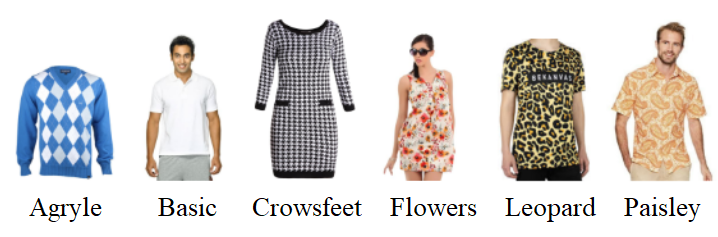
\includegraphics[width=0.48\textwidth]{fig_texture_samples.png}}
\caption{Six different color and texture-based patterns (adapted from \cite{b2}).}
\label{fig_patterns}
\end{figure}

Color and texture feature extraction has been a central topic in Content-Based Image Retrieval (CBIR). Classical color descriptors include color histograms and color moments, which capture statistical properties such as mean, variance, and skewness of color distributions \cite{b24}. For texture representation, methods such as Gabor filters and Local Binary Patterns (LBP) have been widely used to model spatial and structural patterns under varying illumination conditions \cite{b25}.

With the advent of deep learning, CNNs have become the dominant paradigm for visual feature extraction. Baloian et al. \cite{b2} demonstrated that different CNN layers exhibit attribute-specific sensitivity, with early layers being more responsive to color information and deeper layers capturing texture patterns. Other studies have explored multi-layer and multi-attribute feature fusion to build richer representations \cite{b26}. However, the behavior of attribute-specific representations across modern architectures, such as Vision Transformers and State Space Models, remains underexplored.

In this work, we evaluate and compare classical and modern deep architectures for color- and texture-based image classification. We analyze layer-wise representations in CNNs, Vision Transformers, and State Space Models to investigate their sensitivity to visual attributes and the effectiveness of feature fusion strategies.

The dataset used in this study was introduced in \cite{b2} and consists of fashion images collected from Kaggle and online repositories, including hats, dresses, shirts, socks, purses, and scarves. The dataset is divided into two subsets. The first subset contains 1,000 images categorized into 10 color classes (red, black, blue, green, yellow, gray, brown, pink, purple, and orange), as illustrated in Figure~\ref{fig_color_samples}.

\begin{figure}[htbp]
\centerline{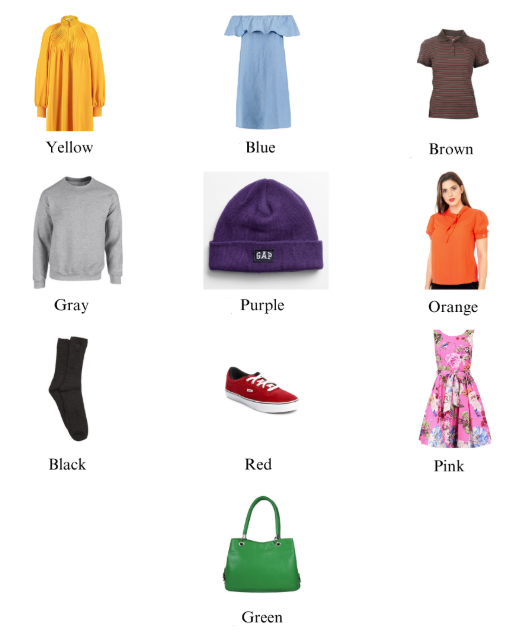
\includegraphics[width=0.48\textwidth]{fig_color_samples.png}}
\caption{Sample images from each class in the color dataset.}
\label{fig_color_samples}
\end{figure}

The second subset contains 1,000 images categorized into 10 texture classes (squared, striped, flowers, leopard, polka dots, basic, paisley, argyle, crowsfeet, and sequin). The objective of this study is to analyze deep metric representations and layer-wise attribute sensitivity for color and texture classification. We evaluate multiple backbone architectures, including ResNet-50 \cite{b4}, VGG-16 \cite{b7}, VMamba \cite{b16}, iBOT \cite{b17}, and LMFCN \cite{b28}, and investigate how different layers contribute to attribute-specific representations and whether feature fusion improves performance.

%The main contributions of this work are: (1) a comparative evaluation of classical and modern deep architectures for attribute-based classification; (2) a layer-wise analysis of color and texture sensitivity across CNNs, Vision Transformers, and State Space Models; and (3) an experimental study on early–deep feature fusion for attribute classification.

The main contributions of this work are summarized as follows:

\begin{itemize}
    \item We provide a comprehensive layer-wise analysis of attribute sensitivity in deep neural networks, evaluating how color and texture representations evolve across depth in classical CNNs, Vision Transformers, and State Space Models.

    \item We present a comparative benchmark of multiple backbone architectures (VGG-16, ResNet-50, iBOT, VMamba, and LMFCN) for color and texture-based image classification, highlighting differences in representational behavior across architectural paradigms.

    \item We experimentally investigate early–deep feature fusion strategies and demonstrate that naive concatenation does not improve attribute classification performance, revealing the limitations of straightforward multi-layer fusion for attribute-specific tasks.

    \item We present attribute-specific feature extraction guidelines, revealing a systematic depth-dependent behavior in which early layers encode color information and deeper layers encode texture information more effectively.
\end{itemize}

This paper is organized as follows. Section~II reviews related work, Section~III describes the methodology, Section~IV presents the evaluated backbone models, Section~V reports experimental results, and Section~VI concludes the paper.



\section{Related Work}

%The use of convolutional networks to represent object similarity is widely used in the literature. Search engines use text searches as their main query method, but searches using image queries are advancing and bringing interesting results to this research field, as presented by the authors in \cite{b2}. In addition to using images, they investigated ResNet-50 layers to determine search by colors and textures. In their research, the authors conclude that the initial layers of the network are better for colors and the deeper layers for textures. In the research, features are extracted with ResNet-50 pre-trained with the ImageNet dataset \cite{b3}. In feature extraction, the first convolutional layer is renamed as Block 1, and residual blocks 2 to 5. At the output of each block, a Global Average Pooling (GAP) layer was applied and the outputs of these layers were used as input to a k-nearest neighbor (KNN) classifier with 5-fold cross-validation.

%In \cite{b10}, the authors employed neural networks to learn a set of features using object categories. In \cite{b11} the authors propose multi-source domain generalization techniques for cross-learning. The authors in \cite{b8} classify plant species by leaf image using the Siamese neural network architecture, combining features from intermediate convolutional layers to improve representations. According to the authors, the combination of features from different layers presents a relevant performance gain and different layers bring different results. In the study by \cite{b9}, the authors used a Siamese neural network to define the similarity index of images of each class through an analysis of the entire leaf and parts of it. In \cite{b13}, the authors present an efficient feature extraction method based on the concept of in-depth texture analysis. For this, wavelet packets and Gabor filter eigenvalues are used for image representation purposes and a partially supervised learning scheme based on K-nearest neighbors. Studies also propose the combination of color and texture features as a feature vector \cite{b14}. Lin et al. \cite{b15} proposed three image content features based on color, texture, and color distribution, such as color co-occurrence matrix (CCM), difference between pixels of scan pattern (DBPSP), and color histogram for K-mean (CHKM) respectively.

%Multi-layer feature fusion has been explored as a strategy to combine representations from different depths of neural networks. The intuition is that early layers capture low-level features (edges, colors) while deeper layers encode high-level semantic information, and combining them could produce richer representations \cite{b26}. Common fusion strategies include early fusion (concatenating features before classification), late fusion (combining classifier outputs), and learned fusion using attention mechanisms \cite{b27}. However, the effectiveness of such approaches for attribute-specific tasks such as color and texture classification remains underexplored.

%Recent advances in deep learning have introduced new architectures that challenge the dominance of Transformers. The Mamba model, proposed by Gu and Dao \cite{b16}, is a notable example. It is a State Space Model (SSM) that achieves linear time complexity in sequence modeling, offering a significant computational advantage over the quadratic complexity of Transformers. Mamba's selective SSMs allow filtering and retrieving information based on content, a capability previously considered a key strength of attention mechanisms. This makes Mamba a promising alternative for various modalities, including language, audio, and genomics, where it has demonstrated state-of-the-art performance.

%In the domain of self-supervised learning for vision, the iBOT model (Image BERT Pre-Training with Online Tokenizer), introduced by Zhou et al. \cite{b17}, has made significant contributions. iBOT uses a masked image modeling (MIM) approach, similar to BERT's masked language modeling, but with a key innovation: an online tokenizer. This allows the model to learn a semantically meaningful visual tokenizer simultaneously with the MIM objective, eliminating the need for a separate pre-training stage for the tokenizer. The Large Margin Fully Convolutional Network (LMFCN) was designed to train Fully Convolutional Networks (FCNs) whose outputs are subsequently used as input features for a large margin classifier, specifically a Support Vector Machine (SVM). During training, the method updates the FCN weights to generate feature representations that maximize the margin between classes, thereby improving SVM classification accuracy.

The use of convolutional neural networks (CNNs) for representing object similarity has been extensively explored in the literature. While text-based queries remain the dominant paradigm in search engines, image-based retrieval has gained increasing attention and demonstrated promising results, particularly in attribute-driven search scenarios \cite{b2}. Baloian et al. \cite{b2} investigated the behavior of ResNet-50 layers for color and texture-based retrieval, showing that early convolutional layers are more sensitive to color information, whereas deeper layers better capture texture patterns. In their framework, features were extracted from ResNet-50 pre-trained on ImageNet \cite{b3}, with Global Average Pooling (GAP) applied to each residual block and k-nearest neighbors (kNN) used for classification with 5-fold cross-validation.

Several studies have explored representation learning for object and attribute recognition. Liang et al. \cite{b10} employed neural networks to learn discriminative features based on object categories, while Gan et al. \cite{b11} proposed multi-source domain generalization techniques for cross-domain attribute learning. Siamese architectures have also been investigated for fine-grained classification tasks; Moresco et al. \cite{b8} demonstrated that combining intermediate-layer features improves plant species classification, highlighting the complementary nature of multi-layer representations. Similarly, Araujo et al. \cite{b9} analyzed similarity across whole and partial leaf structures using Siamese networks.

Classical texture and color descriptors remain relevant for CBIR systems. Irtaza et al. \cite{b13} proposed a texture extraction framework based on wavelet packets and Gabor filter eigenvalues combined with partially supervised kNN classification. Other works investigated joint color–texture feature representations \cite{b14}. Lin et al. \cite{b15} introduced several image content descriptors, including color co-occurrence matrices (CCM), difference between pixels of scan patterns (DBPSP), and color histogram-based clustering (CHKM), demonstrating the importance of multimodal visual attributes.

Multi-layer feature fusion has been proposed to combine representations from different network depths. Early layers typically capture low-level visual cues such as edges and colors, whereas deeper layers encode higher-level semantic information. Fusion strategies include early fusion (feature concatenation), late fusion (decision-level combination), and learned fusion using attention mechanisms \cite{b26,b27}. However, the effectiveness of such approaches for attribute-specific tasks, such as color and texture classification, remains insufficiently studied.

Recent advances in deep learning architectures have challenged the dominance of Transformer-based models. The Mamba architecture, proposed by Gu and Dao \cite{b16}, is a Structured State Space Model (SSM) that achieves linear time complexity in sequence modeling, offering a computational advantage over Transformers’ quadratic complexity. Its selective state-space mechanism enables content-based information filtering and retrieval, making it a promising alternative for multimodal applications, including vision tasks.

In the domain of self-supervised vision learning, the iBOT framework (Image BERT Pre-Training with Online Tokenizer) \cite{b17} introduced a masked image modeling objective with an online tokenizer, allowing simultaneous learning of discrete visual tokens and semantic representations without a separate tokenizer pre-training stage. Additionally, the Large Margin Fully Convolutional Network (LMFCN) framework was proposed to train Fully Convolutional Networks (FCNs) whose learned representations are optimized for large-margin classification using Support Vector Machines (SVMs). During training, FCN parameters are updated to maximize class margins, improving discriminative representation learning for texture and visual pattern classification.

Despite these advances, a systematic layer-wise analysis of attribute-specific representations across modern architectures, including CNNs, Vision Transformers, and State Space Models, remains largely unexplored. This work addresses this gap by evaluating how different architectural paradigms encode color and texture attributes across network depth and by analyzing the impact of multi-layer feature fusion on attribute classification performance.



\section{Applied Methodology}

This study evaluates different deep learning architectures to identify the most effective model for color and texture-based classification. The evaluated models include two classical Convolutional Neural Networks (CNNs), ResNet-50 and VGG-16, and three architectures from recent studies, VMamba, iBOT, and LMFCN, which bring new paradigms for image modeling.

\subsection{ResNet-50}

ResNet-50 \cite{b4} is a 50-layer convolutional neural network that employs residual learning via identity-based skip connections. This design enables the optimization of deep architectures by reformulating the learning objective as residual functions, mitigating gradient degradation and enabling stable training at large depths. ResNet-50 is widely used as a backbone for various computer vision tasks due to its powerful feature extraction capabilities (Figure~\ref{fig_resnet}).


%The Residual Network 50 (ResNet-50), introduced by He et al. \cite{b4}, is a 50-layer deep convolutional neural network. Its central innovation is the use of ``residual blocks'' with skip connections, which allow the model to learn residual functions. This architecture effectively addresses the vanishing gradient problem in very deep networks, enabling the training of models with hundreds or even thousands of layers while maintaining high performance. ResNet-50 is widely used as a backbone for various computer vision tasks due to its powerful feature extraction capabilities (Figure \ref{fig_resnet}).

\begin{figure}[htbp]
\centerline{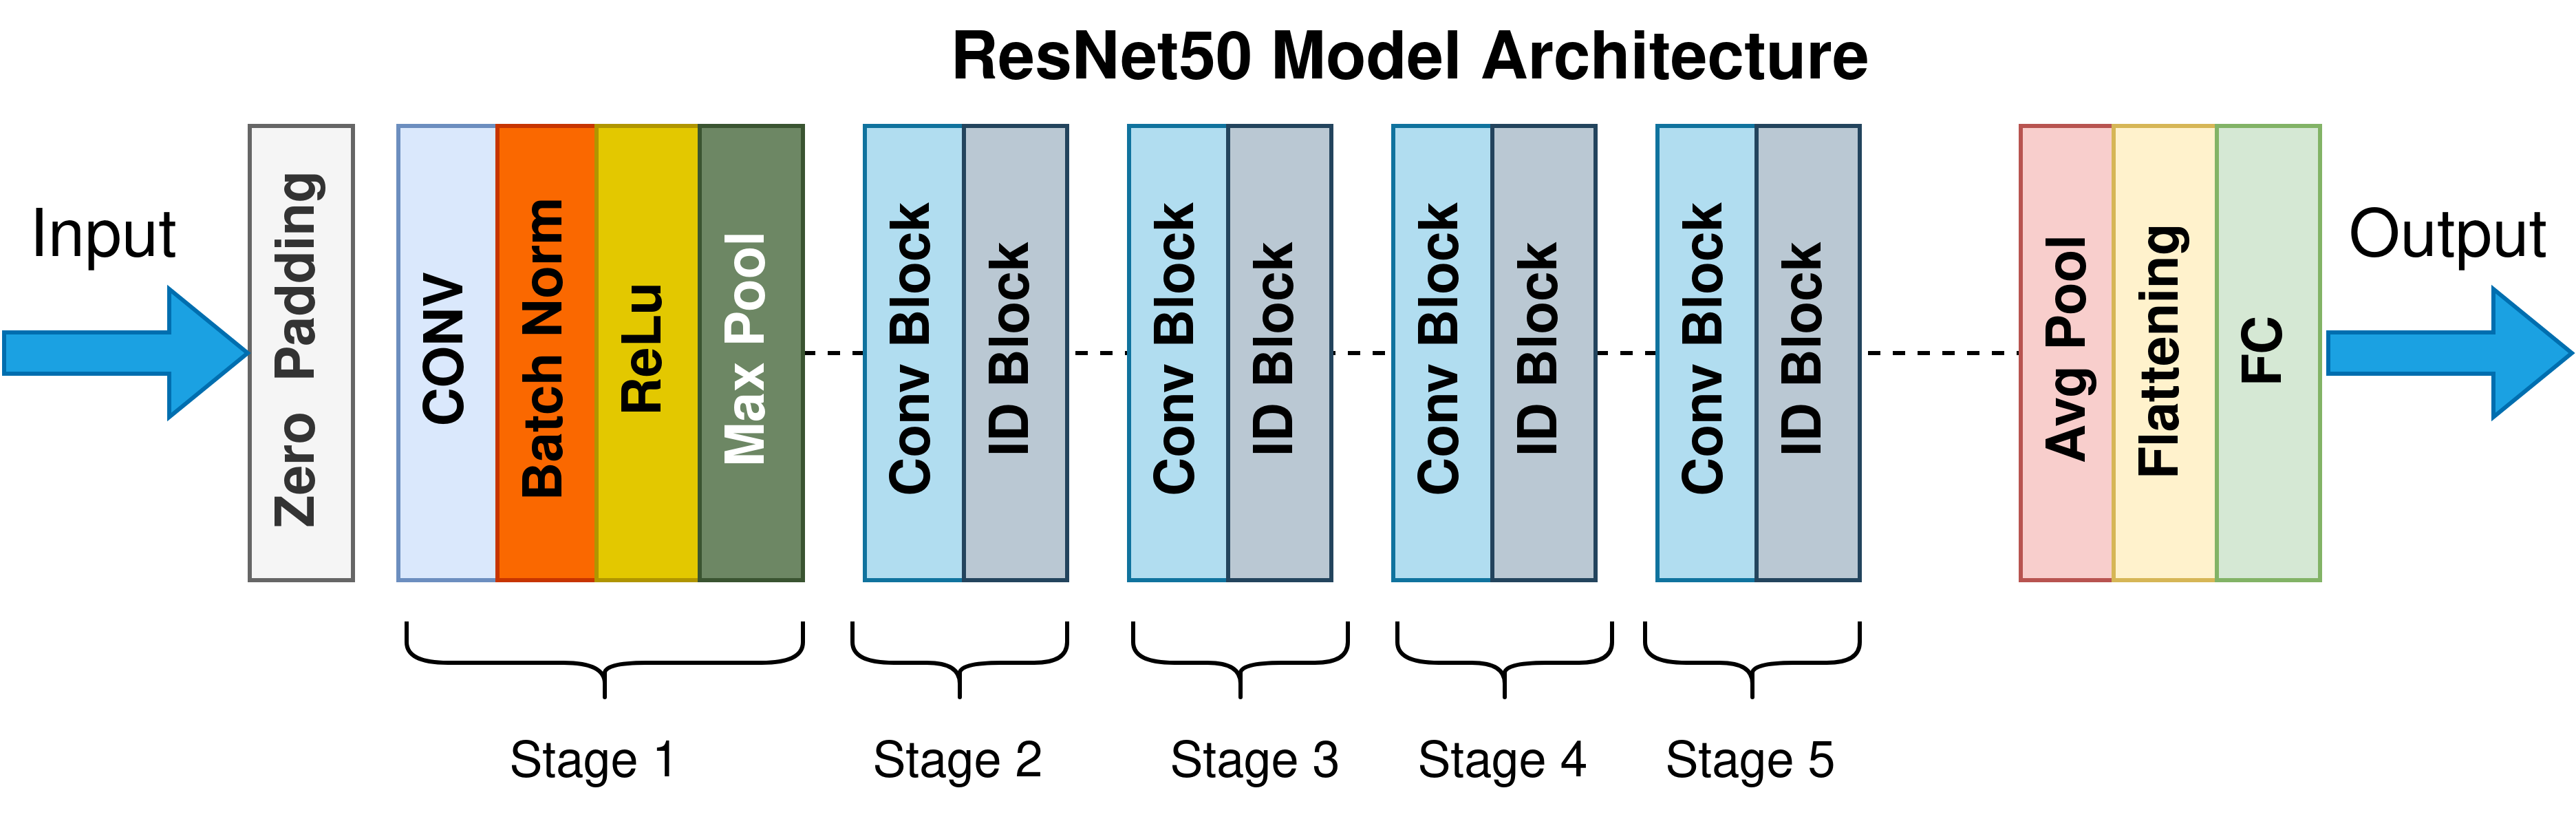
\includegraphics[width=0.48\textwidth]{resnet50.png}}
\caption{ResNet-50 model architecture. Adapted from Mukherjee \cite{b23}, based on the original work by He et al. \cite{b4}.}
\label{fig_resnet}
\end{figure}

\subsection{VGG-16}

VGG-16 \cite{b7} employs a homogeneous architecture with stacked $3 \times 3$ convolutional layers, enabling deep hierarchical feature learning with increased nonlinear expressiveness while maintaining architectural simplicity. It is composed of 16 layers, primarily using small 3x3 convolutional filters stacked on top of each other. This stacking of small filters allows the model to have a large receptive field while maintaining a low number of parameters. Despite its relatively simple architecture, VGG-16 is known for its excellent performance in image classification, and its features have proven to be highly transferable to other tasks (Figure~\ref{fig_vgg}).


%The VGG-16 model, proposed by Simonyan and Zisserman, is a convolutional neural network characterized by its simplicity and depth \cite{b7}. It is composed of 16 layers, primarily using small 3x3 convolutional filters stacked on top of each other. This stacking of small filters allows the model to have a large receptive field while maintaining a low number of parameters. Despite its relatively simple architecture, VGG-16 is known for its excellent performance in image classification, and its features have proven to be highly transferable to other tasks (Figure \ref{fig_vgg}).

\begin{figure}[htbp]
\centerline{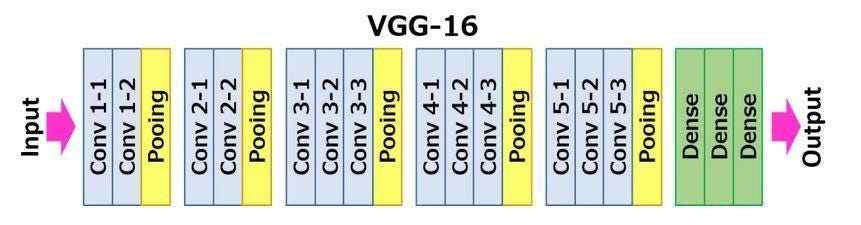
\includegraphics[width=0.48\textwidth]{VGG16.jpg}}
\caption{VGG-16 model architecture, illustrating its sequential structure. Source: Simonyan \& Zisserman \cite{b7}.}
\label{fig_vgg}
\end{figure}

\subsection{VMamba with Convolutional Layers}

VMamba, developed by Gu and Dao \cite{b16}, represents a new class of sequence models based on Structured State Space Models (SSMs). Unlike Transformers, which have quadratic complexity with respect to sequence length, Mamba processes sequences in linear time. It employs a selective scanning mechanism that allows the model to selectively propagate or forget information along a sequence, enabling content-based reasoning. This makes Mamba highly efficient for long sequences and a strong performer across different modalities, including vision, where it can be adapted as a backbone for feature extraction (Figure \ref{fig_mamba}).

\begin{figure}[htbp]
\centerline{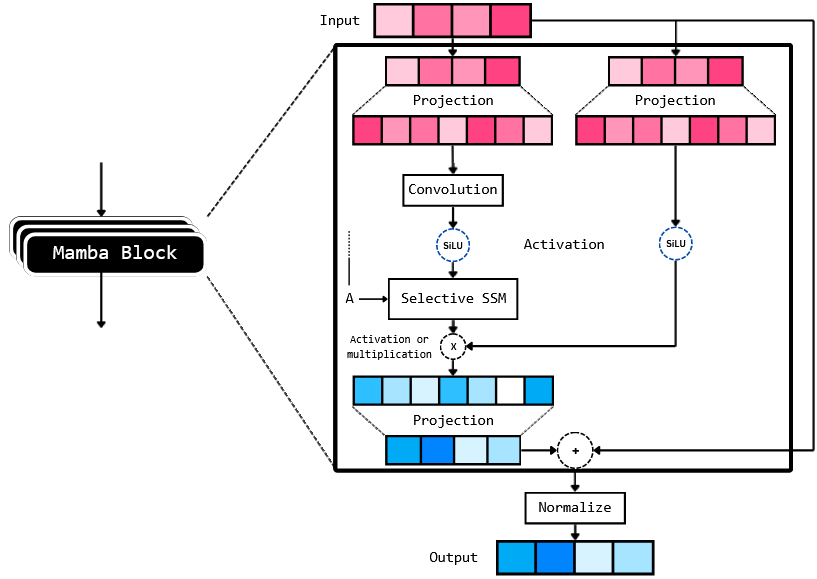
\includegraphics[width=0.48\textwidth]{Vmamba.png}}
\caption{Mamba block diagram, illustrating the selective SSM mechanism. Source: Gu \& Dao \cite{b16}.}
\label{fig_mamba}
\end{figure}

\subsection{iBOT}

The iBOT model (Image BERT Pre-Training with Online Tokenizer), by Zhou et al. \cite{b17}, is a self-supervised learning framework based on Vision Transformers (ViT). It uses a Masked Image Modeling (MIM) objective where parts of an image are masked, and the model must predict the masked content. A key feature of iBOT is its online tokenizer, which learns to create semantically rich visual tokens during the pre-training process. For this study, iBOT is combined with convolutional layers, creating a hybrid model. This approach leverages the strengths of CNNs in capturing local features and fine details, while the Transformer component models global context and relationships between image patches (Figure~\ref{fig_ibot}).

\begin{figure}[htbp]
\centerline{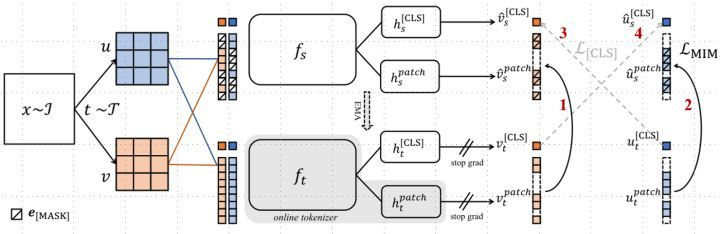
\includegraphics[width=0.48\textwidth]{Ibot.jpg}}
\caption{iBOT framework overview, showing the architecture with an online tokenizer. Source: Zhou et al. \cite{b17}.}
\label{fig_ibot}
\end{figure}

\subsection{LMFCN}

The Large-Margin Fully Convolutional Network (LMFCN) architecture is presented in Figure \ref{fig_lmfcn}. It receives training set images T as input, extracts feature representations using a Fully Convolutional Network (FCN), and uses these features to build the kernel matrix K for an SVM classifier. The FCN can be any convolutional architecture capable of producing a latent representation of the data, such as a TCNN \cite{b28}, ResNet, VGG, or Inception network. Matrix D is a distance matrix defined using the same metric as kernel matrix K and is employed to measure distances between training instances and SVM support vectors. Based on SVM classification results, the distance matrix, and support vectors, FCN parameters are updated using a loss function that increases the penalty for (i) instances that are far from the nearest support vector of the same class, (ii) instances that are close to support vectors of the opposite class, and (iii) instances that are close to non-support instances of the opposite class in the latent representation space. 

\begin{figure}[htbp]
\centerline{\includegraphics[width=0.48\textwidth]{CNNSV4.eps}}
\caption{LMFCN overview. Source: de Matos et al. \cite{b28}.}
\label{fig_lmfcn}
\end{figure}
This method was designed primarily to train small and lightweight FCNs on limited-size datasets, particularly in texture-related classification tasks.
\section{Evaluated Backbone Models}

In this study, classical and modern models were selected. VGG-16 is a classical CNN with 16 weighted layers organized into 5 convolutional blocks using 3×3 filters, each followed by max-pooling, with feature dimensions of 64, 128, 256, 512, and 512. ResNet-50 introduced residual connections (skip connections), enabling deeper networks, consisting of 4 main residual blocks with dimensions of 256, 512, 1024, and 2048. Features are extracted from both CNNs using Global Average Pooling (GAP). These CNNs have been widely used in the literature. In our experiments, we evaluated the outputs of the first five layers of ImageNet-pretrained CNNs. The selection of these layers is based on prior studies reported in the literature \cite{b2,b8}. Features were extracted using Global Average Pooling at the output of each layer. 

For modern architectures, iBOT (Image BERT Pre-Training with Online Tokenizer) is a Vision Transformer pre-trained using self-supervised masked image modeling. In our experiments, we used the ViT-S/16 backbone and extracted features from each of its 12 transformer blocks (Block 0--11) by taking the CLS token embedding (384 dimensions) at the output of each block. VMamba adapts the Mamba architecture, a selective state space model, for visual tasks, achieving linear complexity unlike transformers. We used the VMamba-Tiny variant and extracted features from each of its four stages (Stage 1--4); stage outputs were pooled with Global Average Pooling to obtain a single feature vector per stage (with dimensions 96, 192, 384, and 768, respectively).

LMFCN was evaluated using two fully convolutional network (FCN) architectures: a texture convolutional neural network (TCNN) with three, four, five, and six layers (each consisting of a convolutional layer, a ReLu activation function, and a max pooling) trained from scratch, and a pre-trained ResNet-18 with the final fully connected layers removed. For the ResNet-18 architecture, two configurations were examined: one comprising all residual blocks, called ResNet-18 (4), which uses the first convolutional block and the following four residual blocks, and another, called ResNet-18 (2), retaining only the first convolutional block and the next two residual blocks. FCNs were trained using the LMFCN framework.



\section{Experimental Results}

This section presents the database and experiments conducted to answer the proposed objectives.

\subsection{Experimental Protocol}

The dataset used in this research is the same as that introduced by the authors in \cite{b2}. It consists of 10 classes for color and 10 classes for texture, with 100 images per class, totaling 1,000 images for the color dataset and 1,000 images for the texture dataset. A detailed description of the datasets is provided below:

(a) \textbf{Color dataset}: Contains 100 images of clothing for each of the following color classes: red, black, blue, green, yellow, gray, brown, pink, purple, and orange;

(b) \textbf{Texture dataset}: Contains 100 images of clothing for each of the following texture pattern classes: squared, striped, flowers, leopard, polka dots, basic, paisley, argyle, crowsfeet, and sequin.

The dataset comprises a variety of clothing items, ranging from socks to shirts. The data were split into 70\% for training and 30\% for testing.


%The dataset used in this research was the same used by the authors in \cite{b2}, consisting of 10 classes for color, each containing 100 images, and 10 classes for texture, also with 100 images each, totaling 1000 images for the color set and 1000 images for the texture set. The description of these datasets is given below:

%(a) Color dataset: Contains 100 images of clothing in each of the following colors: red, black, blue, green, yellow, gray, brown, pink, purple, and orange;

%(b) Texture dataset: Contains 100 images of clothing of each of the following texture patterns: squared, striped, flowers, leopard, polka dots, basic, paisley, argyle, crowsfeet, and sequin.

%The dataset is compiled from various clothing items, ranging from socks to shirts. The database was divided into 70\% for training and 30\% for testing.

The evaluation of the feature vectors produced by the previous described models was conducted using a k-nearest neighbors (kNN) classifier with $k=5$ and Euclidean distance, under a 5-fold cross-validation protocol.


\subsection{Classical CNNs Results}

Table~\ref{tab2} presents the classification accuracy obtained for the hidden layers of VGG-16 and residual blocks of ResNet-50. Features were extracted using Global Average Pooling (GAP) and evaluated with k-NN using 5-fold cross-validation as already described. Results reveal a clear relationship between model depth and attribute sensitivity. In VGG-16, Layer 1 achieved the highest color accuracy (95.13\%), with performance progressively decreasing in deeper layers until reaching 55.07\% at Layer 5. Conversely, texture accuracy improved with depth, peaking at Layer 4 (94.73\%). ResNet-50 exhibited similar behavior: Residual Block 2 achieved the best color result (95.87\%), while Residual Block 3 was most effective for texture (93.27\%).

\begin{table}[htbp]
\caption{Accuracy of VGG-16 hidden layers and ResNet-50 Residual Blocks (RB) for color and texture classification.}
\begin{center}
\begin{tabular}{c|c|c|c|c|c}
\hline
\textbf{Layer} & \textbf{Color} & \textbf{Std} & \textbf{Texture} & \textbf{Std} & \textbf{Dim}\\
\hline
VGG-16 Layer 1 & \textbf{95.13} & 0.81 & 70.73 & 2.25 & 64 \\
VGG-16 Layer 2 & 90.27 & 1.27 & 86.60 & 1.57 & 128 \\
VGG-16 Layer 3 & 85.47 & 2.33 & 93.20 & 1.48 & 256 \\
VGG-16 Layer 4 & 71.80 & 2.55 & \textbf{94.73} & 0.74 & 512 \\
VGG-16 Layer 5 & 55.07 & 2.64 & 89.40 & 1.64 & 512 \\
ResNet-50 RB 1 & 95.47 & 0.78 & 83.40 & 1.36 & 256 \\
ResNet-50 RB 2 & \textbf{95.87} & 0.50 & 90.67 & 1.65 & 512 \\
ResNet-50 RB 3 & 88.27 & 1.12 & \textbf{93.27} & 0.25 & 1024 \\
ResNet-50 RB 4 & 59.20 & 3.11 & 86.33 & 0.92 & 2048 \\
\hline
\end{tabular}
\label{tab2}
\end{center}
\end{table}

\subsection{LMFCN Results}

Table~\ref{tab1} presents the results obtained on the texture and color datasets. Results on the texture dataset indicate that increasing the depth of the TCNN leads to improved performance, with classification accuracy consistently increasing as the FCN depth grows. In contrast, the ResNet-18 configuration, including all four Residual Blocks, yielded inferior kNN performance on the texture dataset. 

Results on the color dataset indicate that, compared to the texture dataset, higher classification accuracy is obtained from early network layers. In the ResNet-18 configuration with four Residual Blocks, a degradation in accuracy was observed at the second Residual Block. 

The LMFCN framework with its SVM classifier achieved the best performance on the texture dataset using ResNet-18 with two Residual Block, reaching an accuracy of 96.87\%$\pm$0.9, and on the color dataset using a TCNN with three layers, achieving 97.73\%$\pm$0.95 accuracy.

These results suggest that deeper FCNs are more suitable for texture representation, whereas early layers provide more discriminative features for color classification.


%Table I presents the results obtained on the texture dataset, indicating that increasing TCNN depth leads to better performance, with accuracy consistently increasing as FCN depth increases. In contrast, the ResNet-18 configuration including all four convolutional blocks yielded inferior kNN performance on texture data. Results obtained on the color dataset indicate that, compared to the texture dataset, higher classification accuracy is achieved from early network layers. In the ResNet-18 configuration with four convolutional blocks, a degradation in accuracy was observed at the third layer. LMFCN with its SVM classifier achieved the best performance for the texture dataset for ResNet-18 with two blocks, achieving 96.87\%$\pm$0.9 accuracy, and for the color dataset with TCNN with three layers, with 97.73\%$\pm$0.95 accuracy.

\begin{table}[htbp]
\caption{Accuracy of ResNet-18 Convolutional Block (CB) and Residual Blocks (RB) and TCNN layers using LMFCN for fine-tuning and training respectively.}
\begin{center}
\begin{tabular}{c|c|c|c|c|c}
\hline
\textbf{Method} & \textbf{Color} & \textbf{Std} & \textbf{Texture} & \textbf{Std} & \textbf{Dim}\\
\hline
TCNN3 Layer 1 & 93.33 & 1.13 & 48.73 & 2.28 & 640 \\
TCNN3 Layer 2 & 95.13 & 0.80 & 55.13 & 1.30 & 1280 \\
TCNN3 Layer 3 & \textbf{95.94} & 0.43 & \textbf{58.27} & 1.30 & 640 \\
TCNN4 Layer 1 & 92.67 & 1.53 & 48.67 & 2.28 & 640 \\
TCNN4 Layer 2 & 94.34 & 0.62 & 54.73 & 1.55 & 1280 \\
TCNN4 Layer 3 & 94.20 & 0.38 & 59.73 & 2.26 & 1280 \\
TCNN4 Layer 4 & \textbf{94.80} & 0.65 & \textbf{60.40} & 2.60 & 640 \\
TCNN5 Layer 1 & 93.26 & 1.59 & 48.67 & 3.40 & 640 \\
TCNN5 Layer 2 & \textbf{94.87} & 0.56 & 55.33 & 1.05 & 1280 \\
TCNN5 Layer 3 & 94.33 & 0.71 & 60.80 & 2.61 & 1280 \\
TCNN5 Layer 4 & 94.67 & 0.75 & 62.27 & 3.71 & 1280 \\
TCNN5 Layer 5 & 95.40 & 0.96 & \textbf{62.93} & 1.65 & 640 \\
TCNN6 Layer 1 & 92.87 & 1.49 & 49.33 & 3.04 & 640 \\
TCNN6 Layer 2 & 94.67 & 0.70 & 56.47 & 2.07 & 1280 \\
TCNN6 Layer 3 & \textbf{94.73} & 0.59 & 60.87 & 3.54 & 1280 \\
TCNN6 Layer 4 & 94.53 & 0.87 & 63.47 & 3.82 & 1280 \\
TCNN6 Layer 5 & 94.33 & 1.61 & 63.27 & 2.52 & 1280 \\
TCNN6 Layer 6 & 94.53 & 0.84 & \textbf{64.34} & 2.69 & 640 \\
ResNet-18 (2) CB 0 & 95.00 & 1.05 & 62.73 & 1.01 & 640 \\
ResNet-18 (2) RB 1 & \textbf{96.13} & 0.73 & 84.87 & 1.38 & 640 \\
ResNet-18 (2) RB 2 & 91.93 & 0.98 & \textbf{91.00} & 1.62 & 1280 \\
ResNet-18 (4) CB 0 & 94.53 & 1.57 & 63.67 & 1.68 & 640 \\
ResNet-18 (4) RB 1 & \textbf{95.93} & 0.98 & 84.13 & 1.59 & 640 \\
ResNet-18 (4) RB 2 & 91.07 & 1.16 & 91.20 & 1.39 & 1280 \\
ResNet-18 (4) RB 3 & 89.53 & 1.37 & \textbf{92.47} & 1.48 & 2560 \\
ResNet-18 (4) RB 4 & 75.20 & 1.73 & 86.74 & 1.83 & 5120 \\
\hline
\end{tabular}
\label{tab1}
\end{center}
\end{table}


\subsection{Modern Architectures Results}

The evaluation was extended to modern architectures to verify whether this layer-wise pattern generalizes beyond traditional CNNs. Table~\ref{tab3} shows results for iBOT and VMamba. For iBOT, features were extracted from each transformer block via CLS token, while for VMamba, features were obtained from the output of each processing stage. The iBOT model demonstrated a particularly pronounced gradient: color accuracy decreased from 94.53\% at Block 0 to 62.80\% at Block 11, while texture accuracy increased from 52.20\% to 97.20\% at Block 9 before slightly decreasing in final blocks. This 97.20\% texture accuracy represents the highest value among all evaluated architectures, indicating that self-supervised Vision Transformers capture especially discriminative representations for texture patterns. VMamba showed more compressed behavior due to its four-stage architecture, with Stage 1 achieving the best color accuracy (94.41\%) and Stages 2-3 achieving the best texture accuracy (95.76\%).

\begin{table}[htbp]
\caption{Accuracy of iBOT blocks and VMamba stages for color and texture classification.}
\begin{center}
\begin{tabular}{c|c|c|c|c|c}
\hline
\textbf{Layer} & \textbf{Color} & \textbf{Std} & \textbf{Texture} & \textbf{Std} & \textbf{Dim}\\
\hline
iBOT Block 0 & 94.53 & 1.13 & 52.20 & 2.69 & 384 \\
iBOT Block 1 & 95.40 & 1.27 & 69.87 & 2.28 & 384 \\
iBOT Block 2 & \textbf{95.87} & 1.05 & 79.93 & 2.61 & 384 \\
iBOT Block 3 & 95.20 & 0.83 & 87.87 & 1.44 & 384 \\
iBOT Block 4 & 92.13 & 0.27 & 90.53 & 1.33 & 384 \\
iBOT Block 5 & 88.73 & 0.77 & 91.00 & 2.02 & 384 \\
iBOT Block 6 & 84.93 & 1.24 & 92.20 & 1.85 & 384 \\
iBOT Block 7 & 84.07 & 1.18 & 95.00 & 0.99 & 384 \\
iBOT Block 8 & 76.00 & 0.76 & 96.87 & 0.54 & 384 \\
iBOT Block 9 & 69.93 & 1.97 & \textbf{97.20} & 0.54 & 384 \\
iBOT Block 10 & 66.13 & 3.28 & 96.27 & 0.53 & 384 \\
iBOT Block 11 & 62.80 & 1.73 & 96.00 & 0.87 & 384 \\
VMamba Stage 1 & \textbf{94.41} & 0.52 & 93.86 & 1.07 & 192 \\
VMamba Stage 2 & 93.41 & 0.47 & \textbf{95.76} & 0.84 & 384 \\
VMamba Stage 3 & 78.34 & 3.75 & 95.76 & 0.75 & 768 \\
VMamba Stage 4 & 54.14 & 2.39 & 86.52 & 2.57 & 768 \\
\hline
\end{tabular}
\label{tab3}
\end{center}
\end{table}

Figure~\ref{fig_depth} illustrates the behavior of each architecture with respect to layer depth, clearly showing the inverse pattern between color and texture. In all architectures, color accuracy (red line) tends to decrease with depth, while texture accuracy (blue line) increases until reaching a peak in intermediate or deep layers.

\begin{figure}[htbp]
\centerline{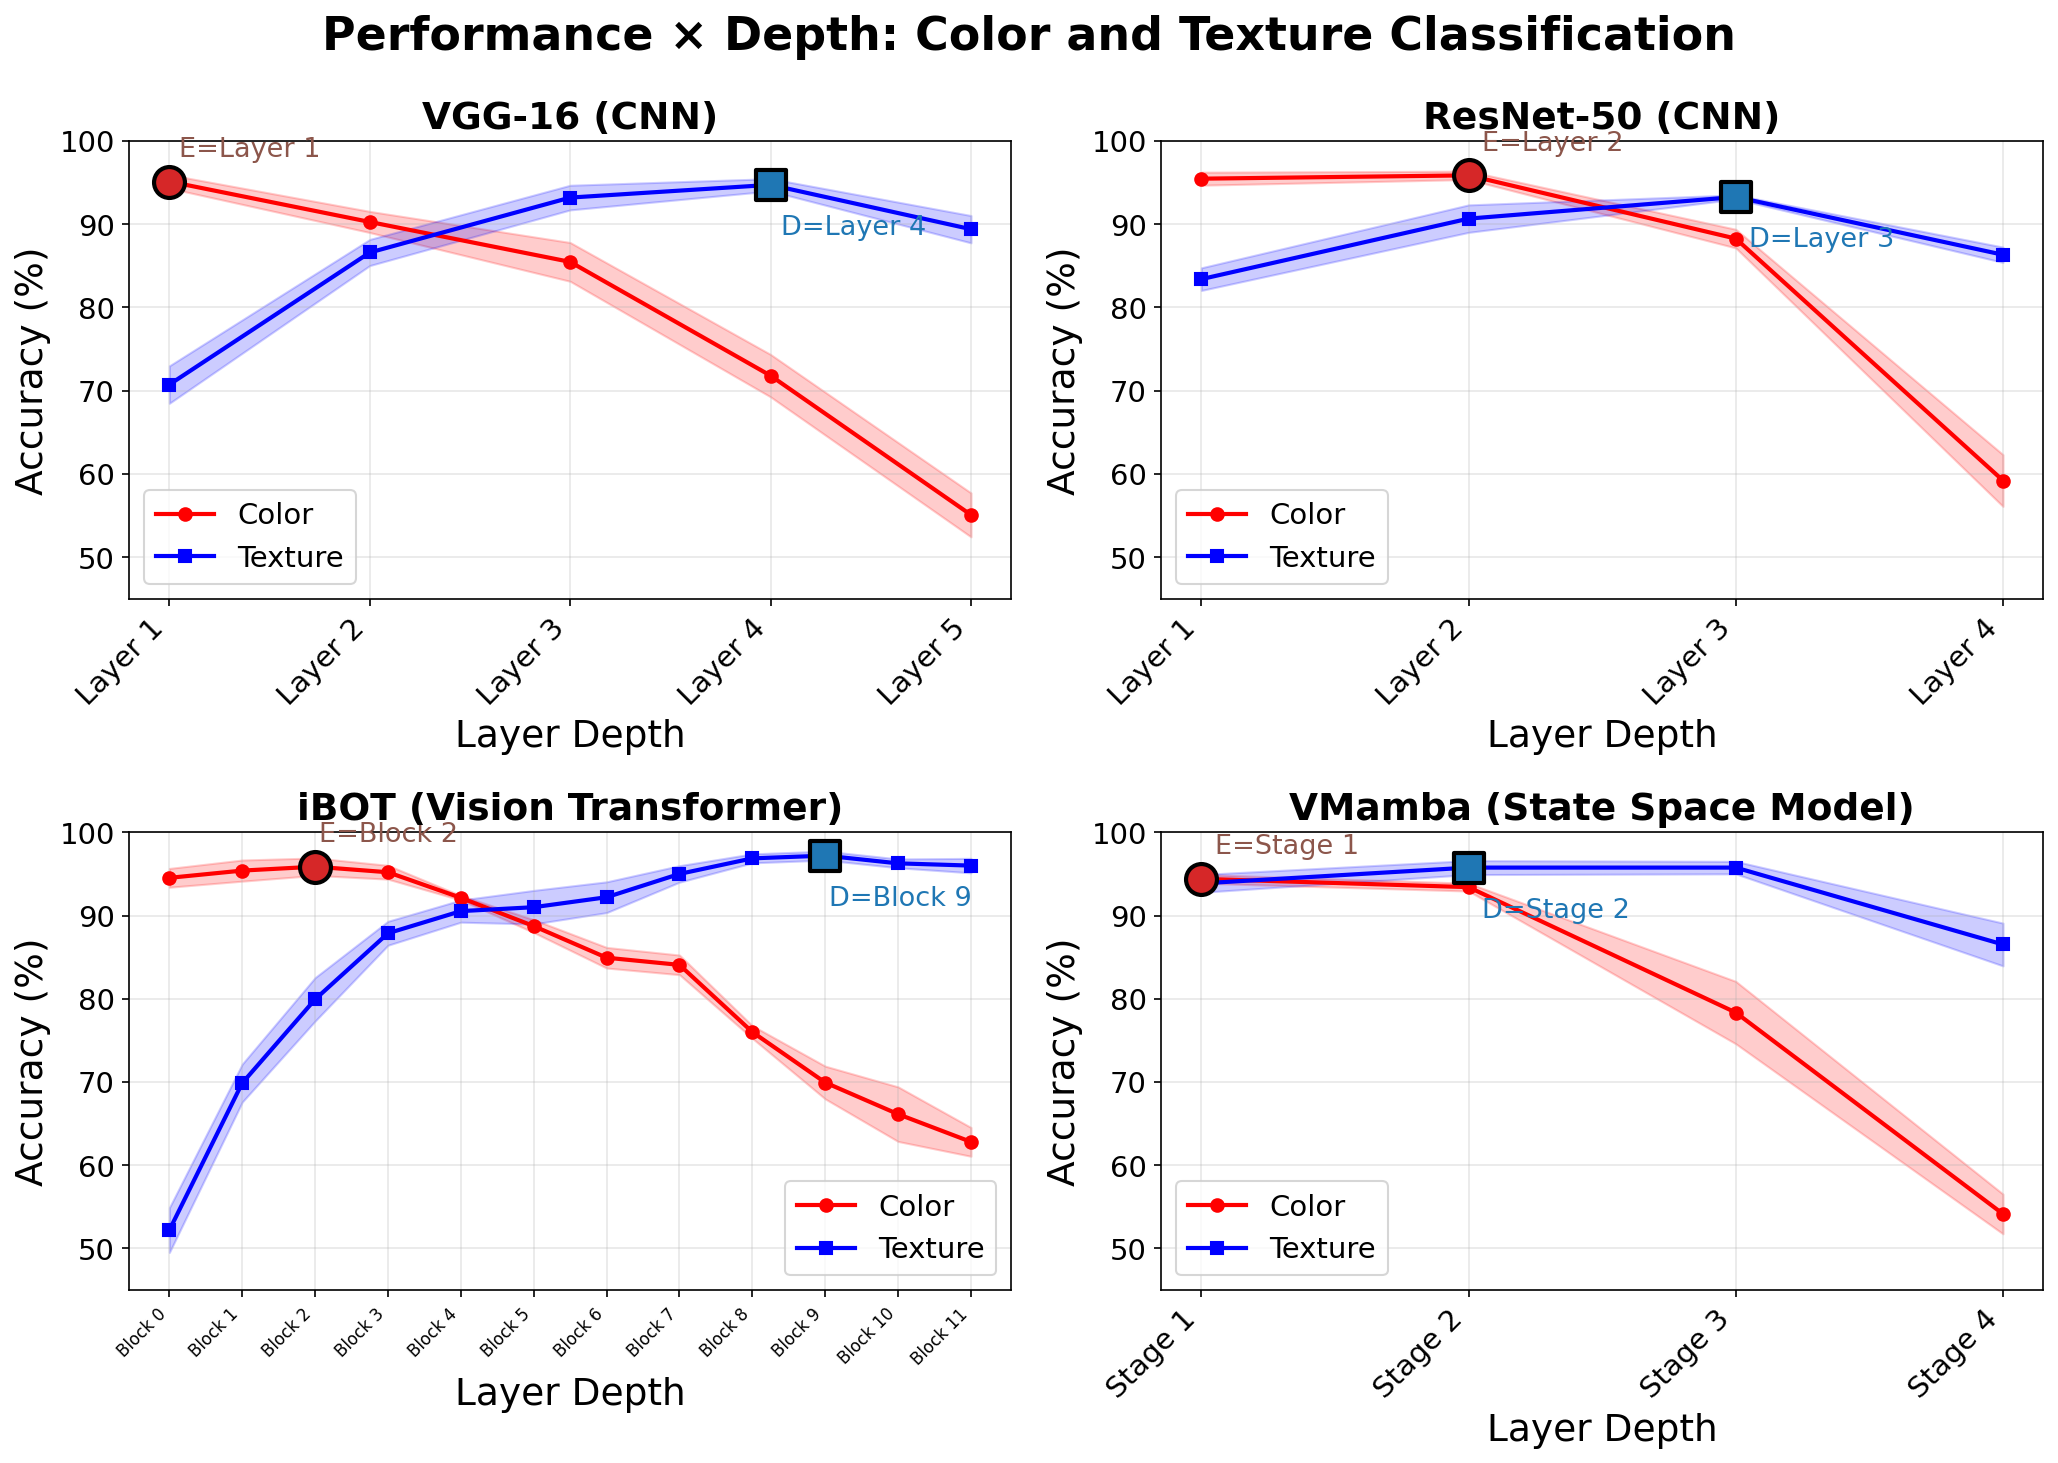
\includegraphics[width=0.48\textwidth]{curvas_desempenho_profundidade.png}}
\caption{Performance × Depth: Color and Texture Classification for VGG-16, ResNet-50, iBOT, and VMamba. Markers indicate the best layers for each attribute (E=color, D=texture).}
\label{fig_depth}
\end{figure}

\subsection{Best Results Summary}

Table~\ref{tab4} consolidates the best results obtained by each architecture. For color classification, ResNet-50 and iBOT tied with 95.87\% accuracy, followed closely by VGG-16 (95.13\%) and VMamba (94.41\%). For texture classification, iBOT stood out with 97.20\%, surpassing VMamba (95.76\%), VGG-16 (94.73\%), and ResNet-50 (93.27\%). These results indicate that while classical CNNs remain competitive for color recognition, modern architectures---particularly self-supervised Vision Transformers---offer advantages for texture-based tasks.

\begin{table}[htbp]
\caption{Best accuracy achieved by each backbone architecture.}
\begin{center}
\begin{tabular}{c|c|c|c|c}
\hline
\textbf{Backbone} & \textbf{Best Color} & \textbf{Color(\%)} & \textbf{Best Texture} & \textbf{Texture(\%)}\\
\hline
VGG-16 & Layer 1 & 95.13 & Layer 4 & 94.73 \\
ResNet-50 & Layer 2 & 95.87 & Layer 3 & 93.27 \\
iBOT & Block 2 & 95.87 & Block 9 & \textbf{97.20} \\
VMamba & Stage 1 & 94.41 & Stage 2 & 95.76 \\
\hline
\end{tabular}
\label{tab4}
\end{center}
\end{table}

Figure~\ref{fig_comparison} presents a direct comparison between all architectures, with normalized depth (0=early layer, 1=deep layer) to allow comparison between models with different numbers of layers. All architectures follow the same general pattern, with iBOT showing the most pronounced gradient.

\begin{figure}[htbp]
\centerline{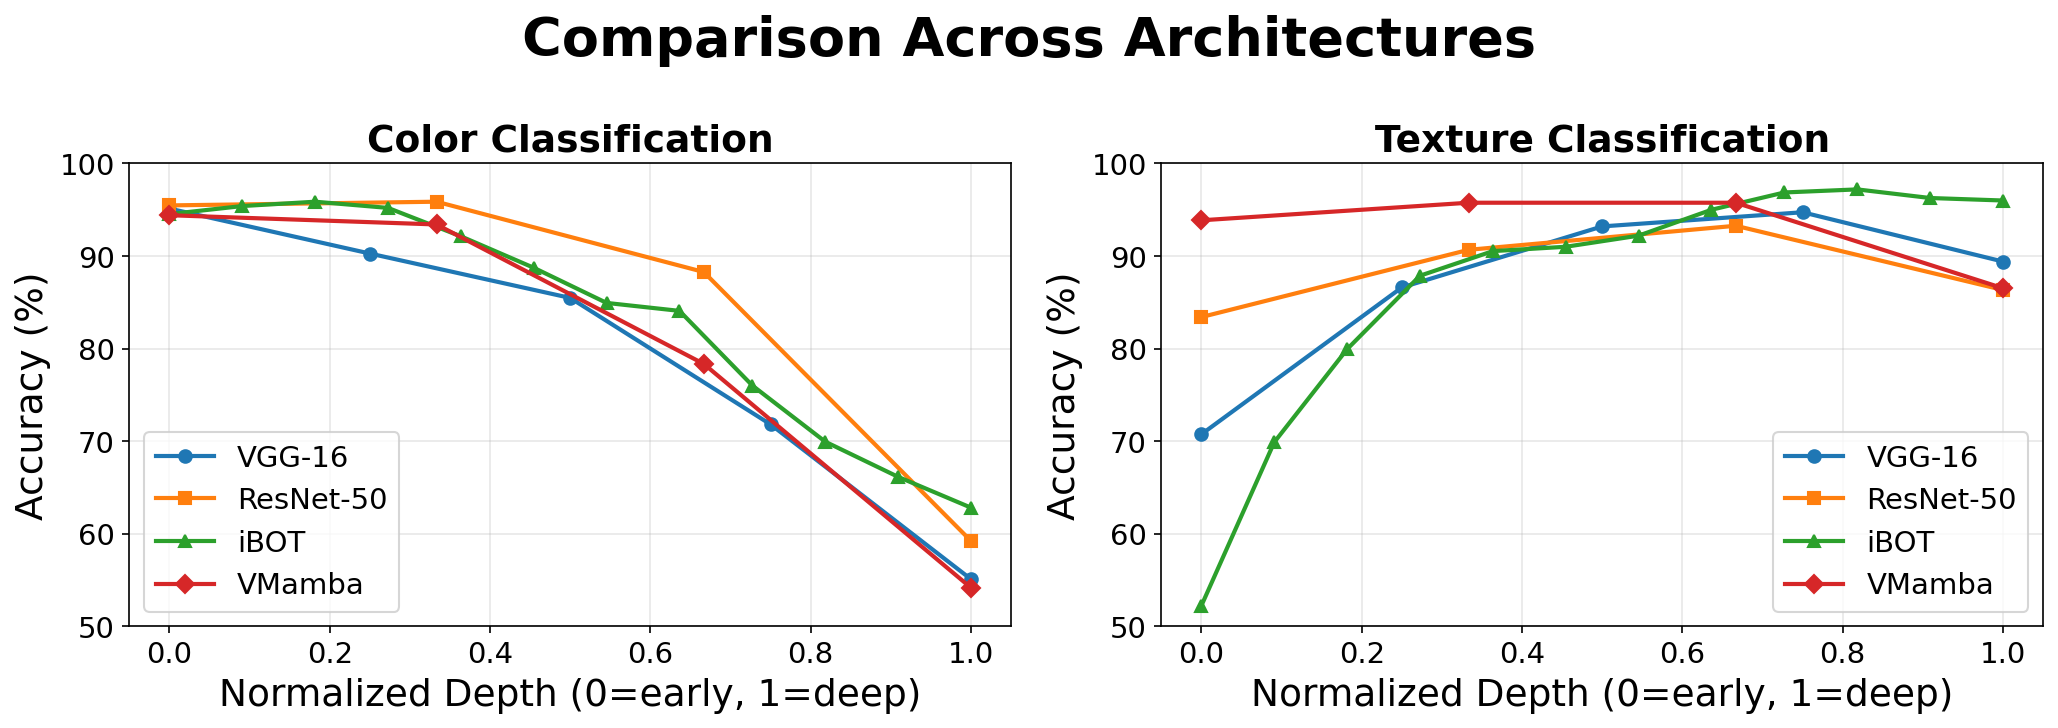
\includegraphics[width=0.48\textwidth]{curvas_comparacao_arquiteturas.png}}
\caption{Comparison Across Architectures: Accuracy vs Normalized Depth for color (left) and texture (right) classification.}
\label{fig_comparison}
\end{figure}

\subsection{Experiment 2: Early-Deep Feature Fusion}

This experiment evaluates whether concatenating features from the best color layer (E) and the best texture layer (D) improves classification performance according to the combination in Table \ref{tab5}. For each backbone, we performed fusion as z = concat(E, D) and evaluated with k-NN (k=5, 5-fold cross-validation).

\begin{table}[htbp]
\caption{Fusion configuration for each backbone.}
\begin{center}
\begin{tabular}{c|c|c|c|c|c}
\hline
\textbf{Backbone} & \textbf{E (Color)} & \textbf{Dim E} & \textbf{D (Texture)} & \textbf{Dim D} & \textbf{Dim z}\\
\hline
VGG-16 & Layer 1 & 64 & Layer 4 & 512 & 576 \\
ResNet-50 & RB 2 & 512 & RB 3 & 1024 & 1536 \\
iBOT & Block 2 & 384 & Block 9 & 384 & 768 \\
VMamba & Stage 1 & 96 & Stage 2 & 192 & 288 \\
\hline
\end{tabular}
\label{tab5}
\end{center}
\end{table}

\begin{table}[htbp]
\caption{Fusion results for color classification.}
\begin{center}
\begin{tabular}{c|c|c|c|c}
\hline
\textbf{Backbone} & \textbf{E (color)} & \textbf{D (texture)} & \textbf{Z (fusion)} & \textbf{$\Delta$}\\
\hline
VGG-16 & \textbf{95.13\%} & 71.80\% & 86.13\% & -9.00\% \\
ResNet-50 & \textbf{95.87\%} & 88.27\% & 94.13\% & -1.73\% \\
iBOT & \textbf{96.93\%} & 81.33\% & 85.13\% & -11.80\% \\
VMamba & \textbf{94.80\%} & 93.93\% & 94.13\% & -0.67\% \\
\hline
\end{tabular}
\label{tab6}
\end{center}
\end{table}

\begin{table}[htbp]
\caption{Fusion results for texture classification.}
\begin{center}
\begin{tabular}{c|c|c|c|c}
\hline
\textbf{Backbone} & \textbf{E (color)} & \textbf{D (texture)} & \textbf{Z (fusion)} & \textbf{$\Delta$}\\
\hline
VGG-16 & 70.73\% & \textbf{94.73\%} & 94.73\% & 0.00\% \\
ResNet-50 & 90.67\% & 93.27\% & \textbf{93.53\%} & +0.27\% \\
iBOT & 78.33\% & \textbf{87.80\%} & 88.07\% & +0.27\% \\
VMamba & 88.40\% & \textbf{94.33\%} & 93.40\% & -0.93\% \\
\hline
\end{tabular}
\label{tab7}
\end{center}
\end{table}

Figure~\ref{fig_fusion} shows the fusion results from Table~\ref{tab6} and Table~\ref{tab7}, comparing the accuracy of color layer features (E), texture layer features (D), and concatenated fusion (Z) for each task and architecture.

\begin{figure}[htbp]
\centerline{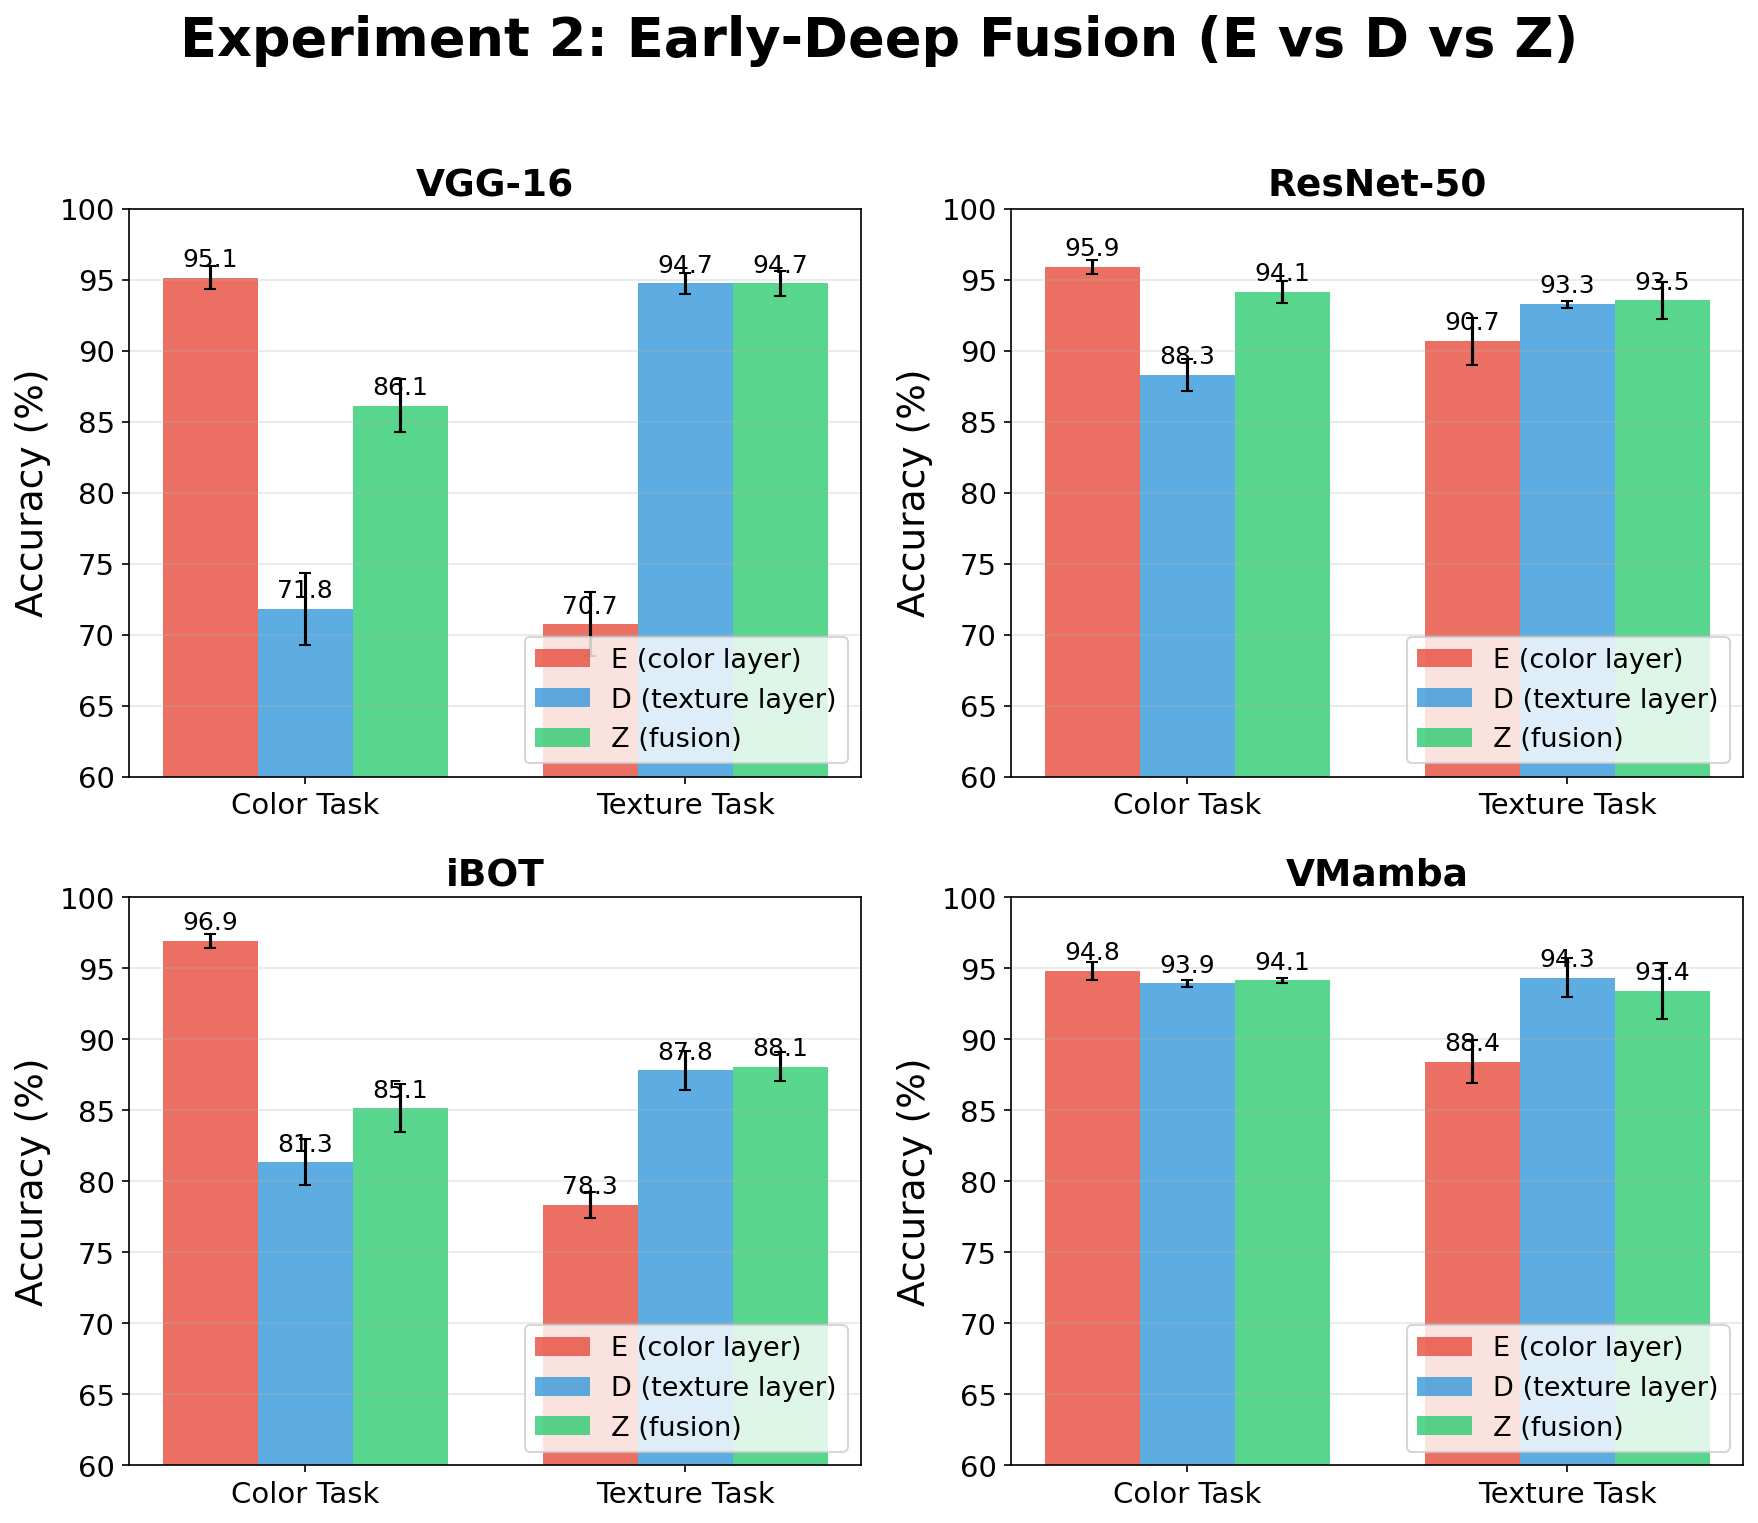
\includegraphics[width=0.48\textwidth]{exp2_fusao_comparacao.png}}
\caption{Experiment 2: Early-Deep Fusion. Comparison between color layer features (E), texture layer features (D), and concatenated fusion (Z) for color and texture classification in each architecture.}
\label{fig_fusion}
\end{figure}

Figure~\ref{fig_impact} presents the fusion impact relative to the best individual layer, clearly showing that concatenation fusion rarely improves performance and frequently degrades it, especially for color classification.

\begin{figure}[htbp]
\centerline{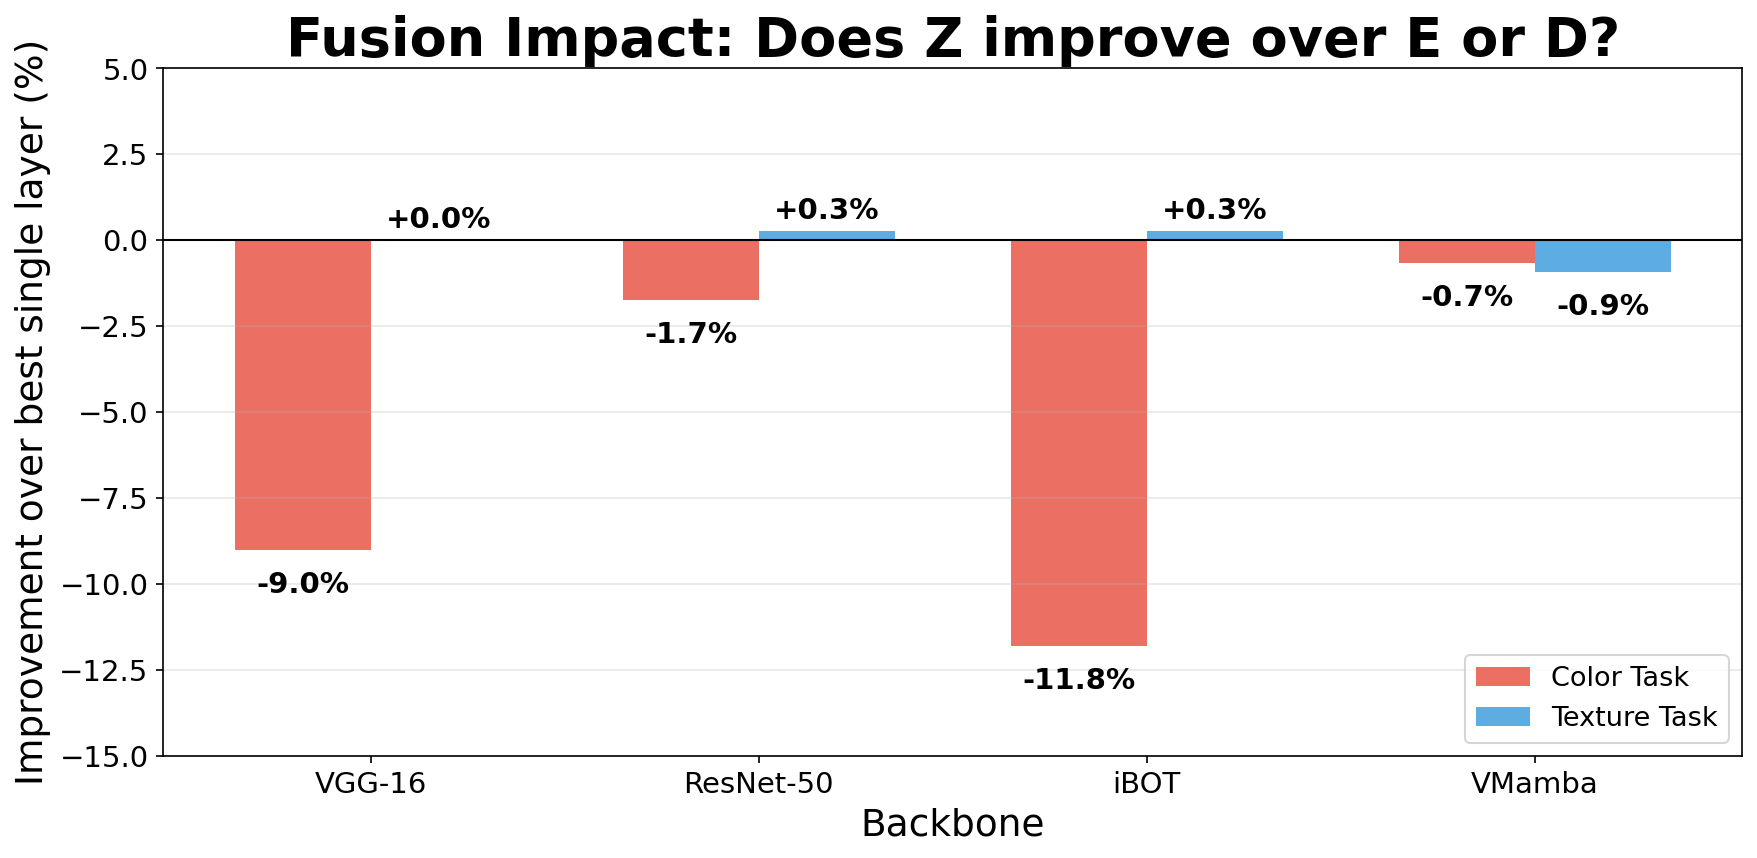
\includegraphics[width=0.48\textwidth]{exp2_fusao_improvement.png}}
\caption{Fusion Impact: Improvement (or degradation) of fusion Z relative to the best individual layer (E or D) for each task.}
\label{fig_impact}
\end{figure}

Fusion results show that simple concatenation generally does not improve classification performance. For color classification, fusion consistently degraded accuracy compared to using the specialized color layer alone (E), with iBOT showing the largest degradation (-11.80\%). For texture classification, results were mixed, with minimal improvements for ResNet-50 and iBOT (+0.27\%) but degradation for VMamba (-0.93\%). These results indicate that specialized single-layer representations are more effective than naive multi-layer fusion.

\subsection{Early-Deep Feature Fusion with LMFCN}

To evaluate whether the pattern observed in previous architectures holds for the LMFCN framework, fusion experiments were also conducted concatenating features from the best layers for color and texture. Table~\ref{tab8} presents the fusion configuration used for each LMFCN architecture. The combination for TCNN3 and TCNN4 used the second best color layer owning to the best layer results being the same for color and texture.

\begin{table}[htbp]
\caption{Fusion configuration for each LMFCN architecture combining color and texture best layers.}
\begin{center}
\begin{tabular}{c|c|c}
\hline
\textbf{Architecture} & \textbf{Fused Layers} & \textbf{Dim z}\\
\hline
TCNN3 & Layer 2 + Layer 3 & 1920 \\

TCNN4 & Layer 3 + Layer 4 & 1920 \\

TCNN5 & Layer 2 + Layer 5 & 1920 \\

TCNN6 & Layer 3 + Layer 6 & 1920 \\

ResNet-18 (2) & RB 1 + RB 2 & 1920 \\

ResNet-18 (4) & RB 1 + RB 3 & 3200 \\
\hline
\end{tabular}
\label{tab8}
\end{center}
\end{table}

The LMFCN fusion results in Tables \ref{tab9} and \ref{tab10} confirm the pattern observed in other architectures. For texture classification, fusion consistently degraded accuracy compared to the best individual layer, with drops ranging from -0.54\% (ResNet-18 with 4 residual blocks) to -4.46\% (TCNN5). For color classification, results were mixed: while most configurations showed degradation, TCNN6 (+0.80\%) and ResNet-18 (2) (+0.20\%) showed small improvements.


\begin{table}[htbp]
\caption{LMFCN fusion results for texture classification.}
\begin{center}
\begin{tabular}{c|c|c|c}
\hline
\textbf{Architecture} & \textbf{Best Layer(\%)} & \textbf{Fusion(\%)} & \textbf{$\Delta$}\\
\hline
TCNN3 & \textbf{58.27} & 56.07 & -2.20\% \\
TCNN4 & \textbf{60.40} & 58.07 & -2.33\% \\
TCNN5 & \textbf{62.93} & 58.47 & -4.46\% \\
TCNN6 & \textbf{64.34} & 62.87 & -1.47\% \\
ResNet-18 (2) & \textbf{91.00} & 89.40 & -1.60\% \\
ResNet-18 (4) & \textbf{92.47} & 91.93 & -0.54\% \\
\hline
\end{tabular}
\label{tab9}
\end{center}
\end{table}


\begin{table}[H] 
\caption{LMFCN fusion results for color classification.}
\begin{center}
\begin{tabular}{c|c|c|c}
\hline
\textbf{Architecture} & \textbf{Best Layer(\%)} & \textbf{Fusion(\%)} & \textbf{$\Delta$}\\
\hline
TCNN3 & \textbf{95.94} & 95.27 & -0.67\% \\
TCNN4 & \textbf{94.80} & 93.20 & -1.60\% \\
TCNN5 & \textbf{95.40} & 95.07 & -0.33\% \\
TCNN6 & 94.73 & \textbf{95.53} & +0.80\% \\
ResNet-18 (2) & 96.13 & \textbf{96.33} & +0.20\% \\
ResNet-18 (4) & \textbf{95.93} & 94.80 & -1.13\% \\
\hline
\end{tabular}
\label{tab10}
\end{center}
\end{table}





Notably, LMFCN's SVM classifier achieved the best absolute results for color (97.73\% with TCNN3) and texture (96.87\% with ResNet-18 with 2 blocks), outperforming concatenation fusion in both cases.




\section{Discussion}

The experimental results presented in this study provide evidence that the layer-wise sensitivity pattern previously observed in classical CNNs extends to modern architectures based on Vision Transformers and State Space Models. Across all evaluated backbones, early layers consistently captured features more suitable for color classification, while deeper layers proved more effective for texture recognition. 

Performance differences between architectures offer insights into their representational characteristics. iBOT's exceptional texture accuracy (97.20\%) suggests that the self-supervised masked image modeling objective encourages learning rich structural representations in deeper layers. The relatively uniform feature dimensionality across iBOT blocks (384 dimensions) contrasts with increasing dimensions in CNNs and VMamba, yet iBOT achieved superior texture discrimination. This indicates that the quality of learned representations, rather than their dimensionality, is the determining factor for texture classification.

The LMFCN method combined with an SVM classifier achieved accuracy values that were comparable, though slightly lower, than the best results obtained by iBOT, with 96.87\% versus 97.20\% on the texture dataset and 97.73\% versus 95.87\% on the color dataset for LMFCN and iBOT, respectively. Notably, the FCNs employed in the LMFCN framework were significantly smaller than those used in the competing methods. As the model size increased, performance degradation was observed, which is consistent with the design characteristics of the LMFCN approach.

The early-deep fusion experiment revealed that simple
concatenation does not improve classification performance. For color classification, merging consistently degraded accuracy compared to using the specialized color layer alone. For texture classification, the results were marginal at best. These results indicate that single-layer specialized representations are more effective than multilayer merging, and more sophisticated merging mechanisms may be needed to take advantage of multilayer capabilities.

The practical implications of these findings are significant. For applications requiring color-based retrieval, features from early layers should be preferred, while texture-based retrieval benefits from deeper layer representations. Furthermore, backbone architecture choice should consider the primary attribute of interest: classical CNNs offer a good balance for color tasks, while iBOT provides substantial advantages for texture-focused applications.


\section{Conclusions}

This study presents a comprehensive evaluation of hidden layer feature extraction across multiple deep learning architectures for color and texture classification in fashion images. We evaluated classical CNNs (VGG-16 and ResNet-50), modern architectures (iBOT and VMamba), and the LMFCN framework.

Experiments confirm that the layer-wise sensitivity pattern observed in previous studies extends to modern Vision Transformers and State Space Models: early layers are more effective for color classification, while deeper layers excel at texture recognition. Among evaluated architectures, iBOT achieved the highest texture accuracy (97.20\% at Block 9), while ResNet-50 and iBOT tied for the best color accuracy (95.87\%). The LMFCN achieved competitive accuracy with both kNN and SVM classifiers, demonstrating its competitiveness among the evaluated methods.

Additionally, simple concatenation fusion of features from the best color and texture layers does not improve performance over specialized single-layer representations, suggesting that more sophisticated fusion mechanisms are needed.

These findings have practical implications for image retrieval systems, suggesting that feature extraction
should be specific to each attribute. Future work will investigate feature matching of optimal layers across different architectures and attention-based merging mechanisms to potentially improve classification performance.


\section*{Acknowledgment}

This work was supported by the Conselho Nacional de Desenvolvimento Científico e Tecnológico (CNPq, Brazil).


\begin{thebibliography}{00}
\bibitem{b1} S. R. Dubey, ``A decade survey of content based image retrieval using deep learning,'' IEEE Trans. Circuits Syst. Video Technol., vol. 32, no. 5, pp. 2687--2704, 2021.
\bibitem{b2} A. Baloian, N. Murrugarra-Llerena, and J. M. Saavedra, ``Scalable visual attribute extraction through hidden layers of a residual convnet,'' arXiv preprint arXiv:2104.00161, 2021.
\bibitem{b3} J. Deng, W. Dong, R. Socher, L.-J. Li, K. Li, and L. Fei-Fei, ``ImageNet: A large-scale hierarchical image database,'' in Proc. IEEE CVPR, 2009, pp. 248--255.
\bibitem{b4} K. He, X. Zhang, S. Ren, and J. Sun, ``Deep residual learning for image recognition,'' in Proc. IEEE CVPR, 2016, pp. 770--778.
\bibitem{b7} K. Simonyan and A. Zisserman, ``Very deep convolutional networks for large-scale image recognition,'' arXiv preprint arXiv:1409.1556, 2014.
\bibitem{b8} M. Moresco, A. D. S. Britto, Y. M. Costa, L. J. Senger, and A. G. Hochuli, ``Combining multi-layer features for plant species classification in a Siamese network,'' in Proc. IEEE SMC, 2022, pp. 2446--2451.
\bibitem{b9} V. M. Ara\'{u}jo, A. S. Britto Jr., L. S. Oliveira, and A. L. Koerich, ``Two-view fine-grained classification of plant species,'' Neurocomputing, vol. 467, pp. 427--441, 2022.
\bibitem{b10} K. Liang, H. Chang, S. Shan, and X. Chen, ``A unified multiplicative framework for attribute learning,'' in Proc. IEEE ICCV, 2015, pp. 2506--2514.
\bibitem{b11} C. Gan, T. Yang, and B. Gong, ``Learning attributes equals multi-source domain generalization,'' in Proc. IEEE CVPR, 2016, pp. 87--97.
\bibitem{b12} S. M. Youssef, ``ICTEDCT-CBIR: Integrating curvelet transform with enhanced dominant colors extraction and texture analysis for efficient content-based image retrieval,'' Comput. Electr. Eng., vol. 38, no. 5, pp. 1358--1376, 2012.
\bibitem{b13} A. Irtaza, M. A. Jaffar, E. Aleisa, and T. S. Choi, ``Embedding neural networks for semantic association in content based image retrieval,'' Multimedia Tools Appl., vol. 72, pp. 1911--1931, 2014.
\bibitem{b14} H. F. Atlam, G. Attiya, and N. El-Fishawy, ``Integration of color and texture features in CBIR system,'' Int. J. Comput. Appl., vol. 164, no. 3, pp. 23--29, 2017.
\bibitem{b15} C. H. Lin, R. T. Chen, and Y. K. Chan, ``A smart content-based image retrieval system based on color and texture feature,'' Image Vis. Comput., vol. 27, no. 6, pp. 658--665, 2009.
\bibitem{b16} A. Gu and T. Dao, ``Mamba: Linear-time sequence modeling with selective state spaces,'' arXiv preprint arXiv:2312.00752, 2023.
\bibitem{b17} J. Zhou et al., ``iBOT: Image BERT pre-training with online tokenizer,'' arXiv preprint arXiv:2111.07832, 2021.
\bibitem{b23} D. Mukherjee, R. Mondal, P. K. Singh, R. Sarkar, and D. Bhattacharjee, ``EnsembleNet: A hybrid approach for vehicle detection,'' Neural Comput. Appl., vol. 32, no. 15, pp. 14207--14228, 2020.
\bibitem{b24} J. Yue, Z. Li, L. Liu, and Z. Fu, ``Content-based image retrieval using color and texture,'' in Proc. ICIG, 2011, pp. 833--837.
\bibitem{b25} E. Prakasa, ``Texture feature extraction by using local binary pattern,'' INKOM J., vol. 1, no. 1, pp. 1--6, 2016.
\bibitem{b26} J. Long, E. Shelhamer, and T. Darrell, ``Fully convolutional networks for semantic segmentation,'' in Proc. IEEE CVPR, 2015, pp. 3431--3440.
\bibitem{b27} Y. Guo, Y. Liu, T. Georgiou, and M. S. Lew, ``A review of semantic segmentation using deep neural networks,'' Int. J. Multimedia Inf. Retr., vol. 7, no. 2, pp. 87--93, 2018.
\bibitem{b28} J. de Matos, L. E. S. de Oliveira, A. D. S. Britto Jr., and A. L. Koerich, ``Large-margin representation learning for texture classification,'' Pattern Recognit. Lett., vol. 170, pp. 39--47, 2023.
\end{thebibliography}

\end{document}
